\subsection{Grid Resolution Sensitivity and Its Impact on Vehicle Classification and Counting}
\label{sec:grid-sensitivity}
\textbf{Selection.} Out-of-fold $J$ ranged only from 0.518 to 0.538 across
the six grids, and the per-fold rule chose $6{\times}8$ in 8 of 10 folds.
On all 26 tuning videos, $J$ was 0.546 ($8{\times}8$), 0.543
($10{\times}12$), 0.543 ($6{\times}8$) and 0.537 ($6{\times}6$), so the tie
rule selected $6{\times}8$ with thresholds Bus if column span $>0.90$ or
both spans $>0.75$, Van if row span $>0.70$ and box aspect $\le2.5$. This
margin is smaller than the fold-to-fold variation; the choice is
reproducible from Eq.~\eqref{eq:objective}, not evidence that
$6{\times}8$ is generally best.

\begin{table}[t]
\centering
\caption{Grid resolution on the 44 unseen-site test videos (per-grid tuned
thresholds; combined lanes). Det.\ rec.: matched ground-truth vehicles;
Frag.: fragmentation; count metrics use downward crossings. FPS: median
of 3 serial trials on the VM. $^{\dagger}$Differs from $6{\times}6$ after
Holm adjustment within the metric ($p<0.05$).}
\label{tab:grid}
\scriptsize
\setlength{\tabcolsep}{2.4pt}
\begin{tabular}{lcccccccc}
\toprule
\textbf{Grid} & \textbf{Mac.-F1} & \textbf{W.-F1} & \textbf{Det.\ rec.} & \textbf{Frag.} & \textbf{Cnt.\ F1} & \textbf{MAE} & \textbf{RMSE} & \textbf{FPS}\\
\midrule
$6{\times}6$     & 0.405 & 0.782 & 0.882 & 1.5\% & 0.314 & 16.0 & 20.4 & 97.2\\
$6{\times}8^{a}$ & 0.416 & 0.799 & 0.892 & 2.3\% & 0.336$^{\dagger}$ & 14.9 & 18.5 & 91.9\\
$8{\times}8$     & 0.402 & 0.813 & 0.894 & 3.8\% & 0.342 & 16.6 & 20.3 & 86.3\\
$10{\times}12$   & 0.430 & 0.815 & 0.908 & 9.5\% & 0.337 & 23.1$^{\dagger}$ & 26.6$^{\dagger}$ & 81.4\\
always-Car       & 0.310 & 0.805 & -- & -- & -- & -- & -- & --\\
\bottomrule
\end{tabular}

\smallskip
\parbox{\columnwidth}{\scriptsize $^{a}$Selected configuration. Always-Car
values vary by $\le0.004$ across grids (row shows $6{\times}8$).}
\end{table}

\begin{table}[t]
\centering
\caption{Test-set classification of the selected $6{\times}8$
configuration (vehicle level, pooled over 44 videos).}
\label{tab:cls}
\scriptsize
\setlength{\tabcolsep}{3.2pt}
\begin{tabular}{lccccccc}
\toprule
\textbf{True} & \multicolumn{3}{c}{\textbf{Predicted}} & \textbf{$n$} & \textbf{Prec.} & \textbf{Rec.} & \textbf{F1}\\
\cmidrule(lr){2-4}
 & Car & Van & Bus & & & & \\
\midrule
Car & 1472 & 126 & 34 & 1632 & 0.889 & 0.902 & 0.895\\
Van & 112 & 23 & 2 & 137 & 0.132 & 0.168 & 0.148\\
Bus & 72 & 25 & 17 & 114 & 0.321 & 0.149 & 0.204\\
\bottomrule
\end{tabular}

\smallskip
\parbox{\columnwidth}{\scriptsize Macro-F1 0.416 vs.\ 0.310 for
always-Car (difference 95\% CI $[0.060, 0.152]$); weighted-F1 0.799 vs.\
0.805 (CI $[-0.022, 0.022]$); accuracy 0.803 vs.\ 0.867. Car$\to$Van
7.7\%, Van$\to$Car 81.8\%, Bus$\to$Car 63.2\%.}
\end{table}

\begin{table*}[t]
\centering
\caption{Counting on the 44 test videos by lane (downward-crossing ground truth; $G_{\uparrow}$:
upward events, never countable). False: unmatched predictions (in brackets: caused by
upward-moving vehicles); Missed: unmatched downward events (in brackets: vehicle not detected
near the line). In the combined scope both ROIs compete for one ground-truth list, so its
TP can exceed the sum of the lanes when a vehicle is counted in the neighbouring ROI.}
\label{tab:count}
\scriptsize
\setlength{\tabcolsep}{3.4pt}
\begin{tabular}{llrrrrrrrcccrr}
\toprule
\textbf{Grid} & \textbf{Scope} & $G_{\downarrow}$ & $G_{\uparrow}$ & $P$ & \textbf{TP} & \textbf{False} & \textbf{Dup.} & \textbf{Missed} & \textbf{Prec.} & \textbf{Rec.} & \textbf{F1} & \textbf{MAE} & \textbf{RMSE}\\
\midrule
$6{\times}6$ & Lane 1 & 501 & 126 & 766 & 217 & 524 (35) & 25 & 284 (14) & 0.283 & 0.433 & 0.343 & 11.4 & 15.0\\
 & Lane 2 & 219 & 434 & 611 & 104 & 483 (125) & 24 & 115 (4) & 0.170 & 0.475 & 0.251 & 10.4 & 14.0\\
 & Combined & 720 & 560 & 1377 & 329 & 974 (172) & 74 & 391 (18) & 0.239 & 0.457 & 0.314 & 16.0 & 20.4\\
\midrule
$6{\times}8$ & Lane 1 & 501 & 126 & 714 & 229 & 464 (35) & 21 & 272 (11) & 0.321 & 0.457 & 0.377 & 10.3 & 13.2\\
 & Lane 2 & 219 & 434 & 604 & 104 & 487 (141) & 13 & 115 (2) & 0.172 & 0.475 & 0.253 & 10.3 & 13.6\\
 & Combined & 720 & 560 & 1318 & 342 & 915 (182) & 61 & 378 (13) & 0.259 & 0.475 & 0.336 & 14.9 & 18.5\\
\midrule
$8{\times}8$ & Lane 1 & 501 & 126 & 765 & 251 & 494 (43) & 20 & 250 (20) & 0.328 & 0.501 & 0.397 & 10.5 & 13.7\\
 & Lane 2 & 219 & 434 & 663 & 107 & 539 (154) & 17 & 112 (3) & 0.161 & 0.489 & 0.243 & 11.4 & 14.9\\
 & Combined & 720 & 560 & 1428 & 367 & 1007 (212) & 54 & 353 (23) & 0.257 & 0.510 & 0.342 & 16.6 & 20.3\\
\midrule
$10{\times}12$ & Lane 1 & 501 & 126 & 931 & 282 & 613 (54) & 36 & 219 (19) & 0.303 & 0.563 & 0.394 & 12.9 & 16.1\\
 & Lane 2 & 219 & 434 & 797 & 125 & 632 (171) & 40 & 94 (2) & 0.157 & 0.571 & 0.246 & 13.9 & 17.8\\
 & Combined & 720 & 560 & 1728 & 413 & 1219 (238) & 96 & 307 (21) & 0.239 & 0.574 & 0.337 & 23.1 & 26.6\\
\bottomrule
\end{tabular}
\end{table*}

\begin{figure}[t]
\centering
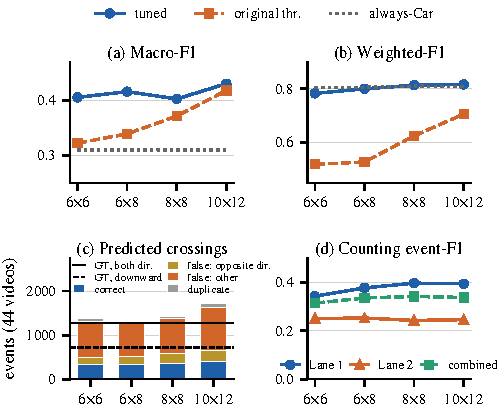
\includegraphics[width=\columnwidth]{figures/fig_grid.pdf}
\caption{Grid resolution on the 44 unseen-site test videos.
(a)~Macro-F1 and (b)~weighted-F1 with the original and the per-grid tuned
thresholds, against always-Car. (c)~Predicted crossings by outcome,
combined lanes, against downward and all trajectory crossings.
(d)~Counting event-F1 per lane.}
\label{fig:grid}
\end{figure}

\textbf{Classification.} With the original thresholds, test macro-F1 rose
with resolution from 0.322 to 0.418 (Fig.~\ref{fig:grid}a); after per-grid
tuning it was 0.402--0.430 for every grid (Table~\ref{tab:grid}), and no
grid differed from $6{\times}6$ (differences $\le0.025$, Holm-adjusted
$p=1.0$). The earlier resolution trend was therefore a calibration effect
of fixed normalized-span thresholds. The tuned classifier beats always-Car
in macro-F1, but its weighted-F1 (0.78--0.82) and accuracy are not higher
(Table~\ref{tab:cls}): it labels 82\% of vans and 63\% of buses as cars
(Van recall 0.17, Bus recall 0.15) and is not a reliable three-class
classifier.

\textbf{Counting.} Table~\ref{tab:count} separates the error sources.
\emph{Directional omissions}: 560 of the 1{,}280 test crossings (44\%)
are upward; 434 of them occur in Lane~2, where upward traffic dominates
(as in the tuning videos: 457 of 739), so the counter never counts that
lane's main direction. \emph{False counts} are the largest error
(915--1{,}219); 18--21\% come from upward-moving vehicles whose cluster
centroid jumps downward across the line, and at $6{\times}8$, 701 of the
976 unmatched predictions overlap no annotated vehicle (spurious motion
clusters). \emph{Missed downward counts} are mostly association failures:
at $6{\times}8$, 365 of 378 missed vehicles were detected near the line,
but no track crossed it (for example because the track started below the
line or was split). \emph{Duplicates} (54--96) are highest at
$10{\times}12$. Track association is weak at every resolution: a
ground-truth vehicle is covered by 2.5--3.1 tracks on average, and
69--75\% of vehicles have at least one identity switch.

With finer grids, correct counts rise (329 to 413) but false and
duplicate counts rise faster (1{,}048 to 1{,}315), so the per-video
error grows at $10{\times}12$: MAE $+7.1$ (95\% CI $[5.4, 8.4]$,
Holm-adjusted $p=0.010$) and RMSE $+6.2$ ($p=0.013$) relative to
$6{\times}6$. $6{\times}8$ raises counting F1 by 0.022 ($[0.012, 0.030]$,
$p=0.012$), a statistically supported but small gain. Its objective gain
($J$: $+0.011$, nominal $p=0.03$) does not survive the Holm adjustment
($p=0.09$), and $10{\times}12$ does not change $J$ ($+0.0004$, $p=0.96$).
Corrected over all 18 tests, no difference reaches $p<0.05$ (smallest:
$10{\times}12$ MAE, $p=0.058$). In practical terms, the macro-F1
differences are small, while 7 extra count errors per video at
$10{\times}12$ (+44\%) are large.

\textbf{Why fragmentation grows.} After the per-cell dilation, a single
pixel above threshold fills its cell, so the 100\,px$^2$ contour filter
never takes effect. As cells shrink (from $73{\times}23$ to
$36{\times}14$\,px), the interiors of vehicles, which frame differencing
leaves unmarked, become empty cells that split a vehicle into several
clusters. In separately run diagnostic variants on the tuning videos,
bridging a single empty cell row removed 87--89\% of the fragmentation and
8-connectivity removed 35--40\%. Neither improved classification.

